%%%%%%%%%%%%%%%%%%%%%%%%%%%%%%%%%%%%%%%%%
% a0poster Portrait Poster
% LaTeX Template
% Version 1.0 (22/06/13)
%
% The a0poster class was created by:
% Gerlinde Kettl and Matthias Weiser (tex@kettl.de)
% 
% This template has been downloaded from:
% http://www.LaTeXTemplates.com
%
% License:
% CC BY-NC-SA 3.0 (http://creativecommons.org/licenses/by-nc-sa/3.0/)
%
%%%%%%%%%%%%%%%%%%%%%%%%%%%%%%%%%%%%%%%%%
% Perrinet18gdr
%----------------------------------------------------------------------------------------
%	PACKAGES AND OTHER DOCUMENT CONFIGURATIONS
%----------------------------------------------------------------------------------------
\newcommand{\Author}{Laurent U.~Perrinet$^1$}%
\newcommand{\Address}{$^1$~Institut de Neurosciences de la Timone, CNRS / Aix-Marseille Universit\'e - Marseille, France}%
\newcommand{\Website}{http://invibe.net/LaurentPerrinet}%
\newcommand{\Title}{A low-cost, accessible eye tracking framework}%
\newcommand{\Email}{laurent.perrinet@univ-amu.fr}%

\documentclass[a0,portrait]{a0poster}

\usepackage{multicol} % This is so we can have multiple columns of text side-by-side
\columnsep=100pt % This is the amount of white space between the columns in the poster
\columnseprule=0pt % This is the thickness of the black line between the columns in the poster

\usepackage[svgnames]{xcolor} % Specify colors by their 'svgnames', for a full list of all colors available see here: http://www.latextemplates.com/svgnames-colors

\usepackage{times} % Use the times font
%\usepackage{palatino} % Uncomment to use the Palatino font

\usepackage{graphicx} % Required for including images
\graphicspath{{figures/}} % Location of the graphics files
\usepackage{booktabs} % Top and bottom rules for table
\usepackage[font=small,labelfont=bf]{caption} % Required for specifying captions to tables and figures
\usepackage{amsfonts, amsmath, amsthm, amssymb} % For math fonts, symbols and environments
\usepackage{wrapfig} % Allows wrapping text around tables and figures

\usepackage{natbib}
\begin{document}

%----------------------------------------------------------------------------------------
%	POSTER HEADER 
%----------------------------------------------------------------------------------------

% The header is divided into two boxes:
% The first is 75% wide and houses the title, subtitle, names, university/organization and contact information
% The second is 25% wide and houses a logo for your university/organization or a photo of you
% The widths of these boxes can be easily edited to accommodate your content as you see fit

\begin{minipage}[b]{0.75\linewidth}
%\VeryHuge
\Huge \color{Navy} \textbf{\Title} \color{Black}\\ % Title
%\Huge\textit{Country Update}\\[2.4cm] % Subtitle
\huge \textbf{\Author} \\[0.5cm] % Author(s)
\huge \Address\\[0.4cm] % University/organization
\Large \texttt{\Email} \\
\end{minipage}
%
\begin{minipage}[b]{0.25\linewidth}

\includegraphics[width=13cm]{Logo_int.png}\ 

\includegraphics[width=10.5cm]{Logo_amu.png}\\
\end{minipage}

\vspace{1cm} % A bit of extra whitespace between the header and poster content

%----------------------------------------------------------------------------------------

\begin{multicols}{3} % This is how many columns your poster will be broken into, a portrait poster is generally split into 2 columns

%----------------------------------------------------------------------------------------
%	ABSTRACT
%----------------------------------------------------------------------------------------

\color{Navy} % Navy color for the abstract

\begin{abstract}
Recording eye movements is a technique that attracts an increasing number of scientists, but also in the general public. Indeed, this allows to quantitatively measure a number of useful dimensions of perception and behavior in general. However, most existing trackers rely on expensive or technically complex solutions. Here, we propose a simple framework to record eye movements using any camera, such as a webcam. As a proof of concept, the recorded image is processed in real-time to detect from a simple sub-set of eye movements : left, center, right or blink. The processing is based on two stages. First, we use a pre-trained computer vision algorithm to extract the image of the face. Second, we used a classical deep-learning architecture to learn to classify these sub-images. This network is a 3 layered convolutional neural network, for which we optimized performance as measured by the accuracy with cross-validation on a wide range of the network's hyper-parameters. Over a dataset of more than 1000 images, this network achieves an average accuracy of approximately 97\%. We also provide with an integration with the psychopy library which shows that frames can be processed on a standard laptop at a rate of approximately 25Hz.
\end{abstract}

%----------------------------------------------------------------------------------------
%	INTRODUCTION
%----------------------------------------------------------------------------------------
\color{Black} % SaddleBrown color for the introduction
\section*{Why another eye tracker?}
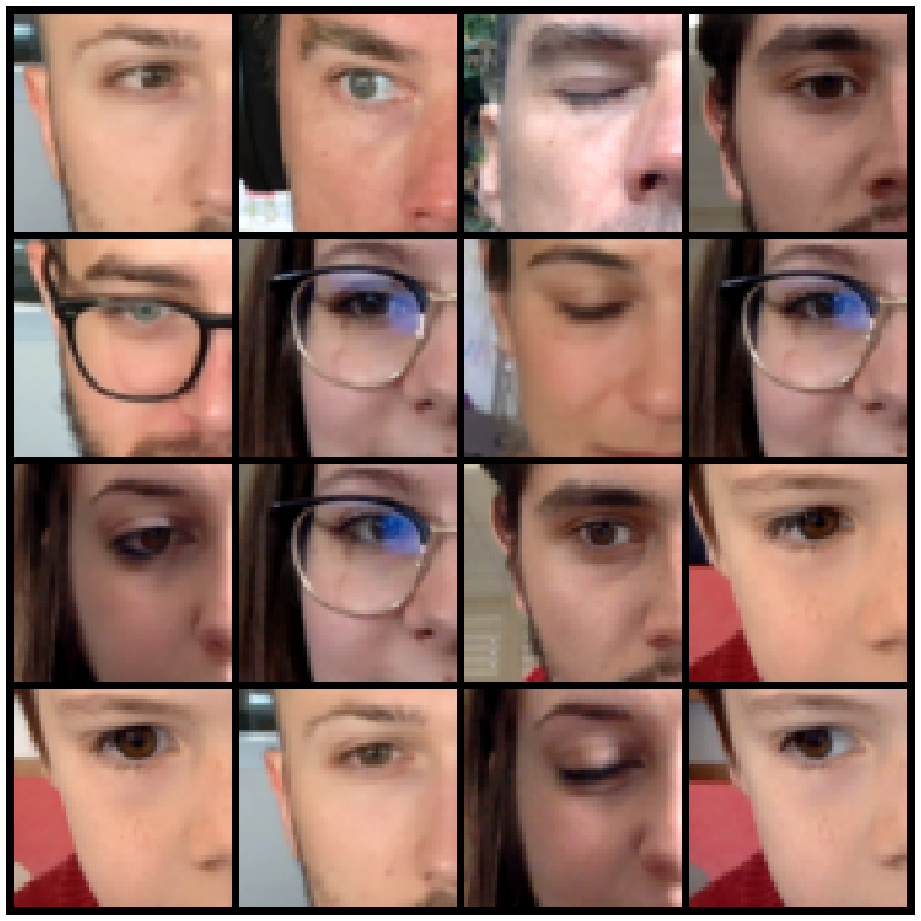
\includegraphics[width=1.\linewidth]{dataset.pdf}
%\captionof{figure}{\color{DarkSlateGray} We investigated the performance of a novel, low-cost, low-precision eye tracker.}
%\end{center}%\vspace{1cm}


\includegraphics[width=1.\linewidth]{accuracy.pdf}
\captionof{figure}{\color{DarkSlateGray} We investigated the performance of a novel, low-cost, low-precision eye tracker.}
%----------------------------------------------------------------------------------------


\end{multicols}


\color{Black} % DarkSlateGray 
\begin{minipage}{0.67\linewidth}
the content
\section*{Recognition model}
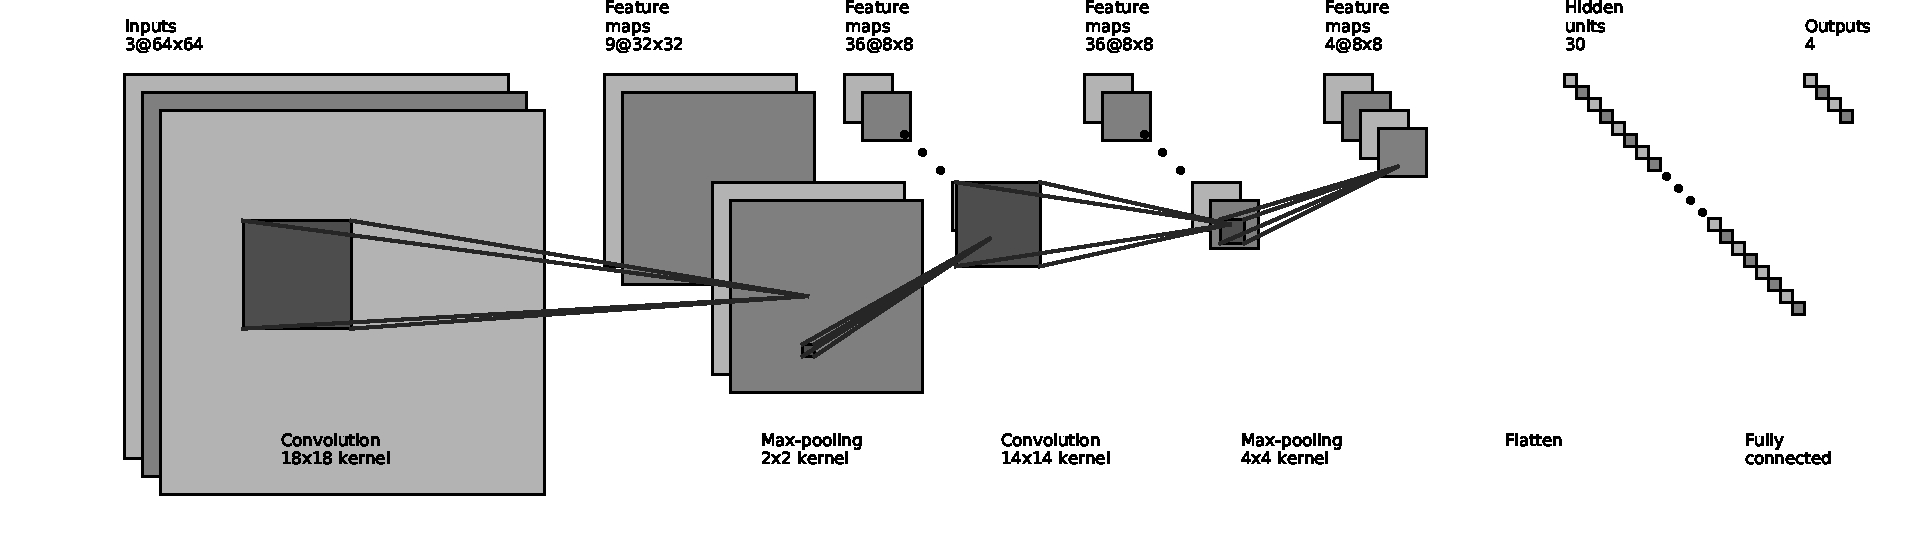
\includegraphics[width=1\linewidth]{CNN.pdf}
%----------------------------------------------------------------------------------------
\end{minipage}
\begin{minipage}{0.3\linewidth}
\captionof{figure}{\color{DarkSlateGray} The architecture of the original convolutional neural network, as introduced by LeCun et al. (1989), alternates between convolutional layers including rectifying non-linearities and max-pooling layers layers. The feature maps of the final subsampling layer are then fed into two layers of fully connected neurons. The output layer uses softmax activation functions to generate a decision. Our model was trained on more than 1000 images taken from a webcam. Accuracy was tested on 20 cross-validations.
}
\end{minipage}\hfil



\begin{multicols}{3} % This is how many columns your 
\section*{Quantitative performance}

\color{Navy} % SaddleBrown color for the conclusions to make them stand out

\section*{Conclusions}


\color{Black} % Set the color back to DarkSlateGray for the rest of the content

\section*{Additional resources}

\begin{minipage}{0.3\linewidth}

\includegraphics[width=1.\linewidth]{GitQR.png}
\end{minipage}\hfil
\begin{minipage}{0.67\linewidth}
The model and data are open-source. You can either flash the code or go to www.github.com/hugoladret/InternshipM1 to get them.
\end{minipage}

 %----------------------------------------------------------------------------------------
%	REFERENCES
%----------------------------------------------------------------------------------------
%\nocite{*} % Print all references regardless of whether they were cited in the poster or not
\bibliographystyle{plain} % Plain referencing style
\bibliography{Perrinet18gdr} % Use the example bibliography file sample.bib
%----------------------------------------------------------------------------------------

\end{multicols}
\end{document}

